%%%%%%%%%%%%%%%%%%%%%%%%%%%%%%%%%%%%%%%%%%%%%%%%%%%%%%%%%%%%%%%%%%%%%%%%%%
%%%%%                         CHAPITRE 3                            %%%%%%
%%%%%%%%%%%%%%%%%%%%%%%%%%%%%%%%%%%%%%%%%%%%%%%%%%%%%%%%%%%%%%%%%%%%%%%%%%

\lhead[\fancyplain{}{\leftmark}]%Pour les pages paires \bfseries
      {\fancyplain{}{}} %Pour les pages impaires
\chead[\fancyplain{}{}]%
      {\fancyplain{}{}}
\rhead[\fancyplain{}{}]%Pour les pages paires 
      {\fancyplain{}{\rightmark}}%Pour les pages impaires \bfseries
\lfoot[\fancyplain{}{}]%
      {\fancyplain{}{}}
\cfoot[\fancyplain{}{\thepage}]%\bfseries
      {\fancyplain{}{\thepage}} %\bfseries
\rfoot[\fancyplain{}{}]%
     {\fancyplain{}{\scriptsize}}


%%%%%%%%%%%%%%%%%%%%%%%%%%%%%%%%%%%%%%%%%%%%%%%%%%%%%%%%%%%%%%%%%%%%%%%%%%
%%%%%                      Start part here                          %%%%%%
%%%%%%%%%%%%%%%%%%%%%%%%%%%%%%%%%%%%%%%%%%%%%%%%%%%%%%%%%%%%%%%%%%%%%%%%%%

\chapter{Proposed solution: Pose2Sim Python package}
\label{ch:3}

%==============================================================================	Résumé du chapitre

\begin{center}
\rule{0.7\linewidth}{.5pt}
\begin{minipage}{0.7\linewidth}
\smallskip

\textit{We propose the Pose2Sim python package, as an alternative to the more usual marker-based motion capture methods.Pose2Sim stands for "OpenPose to OpenSim", as it uses OpenPose inputs (2D keypoints coordinates obtained from multiple videos) and leads to an OpenSim result (physically consistent full-body 3D joint angles). Code is available at \url{https://github.com/perfanalytics/pose2sim}. \newline \newline
This chapter is adapted from the article published in the Journal of Open Source Software: "Pose2Sim: An Open-source Python Package for multiview markerless kinematics" \cite{Pagnon2022b}.}

%\smallskip
\end{minipage}
\smallskip
\rule{0.7\linewidth}{.5pt}
\end{center}

\minitoc
\newpage


% Sections 
% Intro: motivation, workflow, install, demo
% Method details: Project, 2D kpt detec, calib, track, trig, filt & others, opensim scale & IK

% Mix JOSS & github


\section{Introduction to the workflow}

Although some developments are relevant to both, specifics differ between medicine and the sports field. In this regard and as stated in the \nameref{sec:statement of need}, marker-based methods are not well suited for sports motion analysis \cite{Colyer2018}. In sports, capture should not hinder the movement. Placing markers on the naked body takes time and is cumbersome, therefore markerless approaches are favored. Sports environments are usually much more challenging than lab settings: frequent occlusions, fast and unusual movements, and complex background make it important to resort to using multiple view points, from RGB rather than RGB-D cameras, processed with machine learning methods. Competition conditions are often fast-paced and congested, so a light-weight, fast, and easy to set up system is relevant. However, as coaches and athletes usually need a mere feedback rather than a definitive diagnosis, they don't need as thorough of an accuracy as physicians. Ideally, results should be given in real time, and they should be more visual than graphs of time series. Moreover, 3D kinematics are more relevant than 2D sagittal plane kinematics; and full-body analysis (including upper-limb) is desired.

We propose the Python package Pose2Sim \cite{Pagnon2022b}, which aims to deal with these constraints. It provides a framework for 3D markerless kinematics, as an alternative to the more usual marker-based motion capture methods. Pose2Sim stands for "OpenPose to OpenSim", as it uses OpenPose inputs (2D coordinates obtained from multiple videos) \cite{Cao2019} and leads to an OpenSim result (full-body 3D joint angles) \cite{Delp2007,Seth2018}. Pose2Sim is accessible at \url{https://github.com/perfanalytics/pose2sim}.

\begin{figure}[hbtp]
	\centering
	\def\svgwidth{1\columnwidth}
	\fontsize{10pt}{10pt}\selectfont
	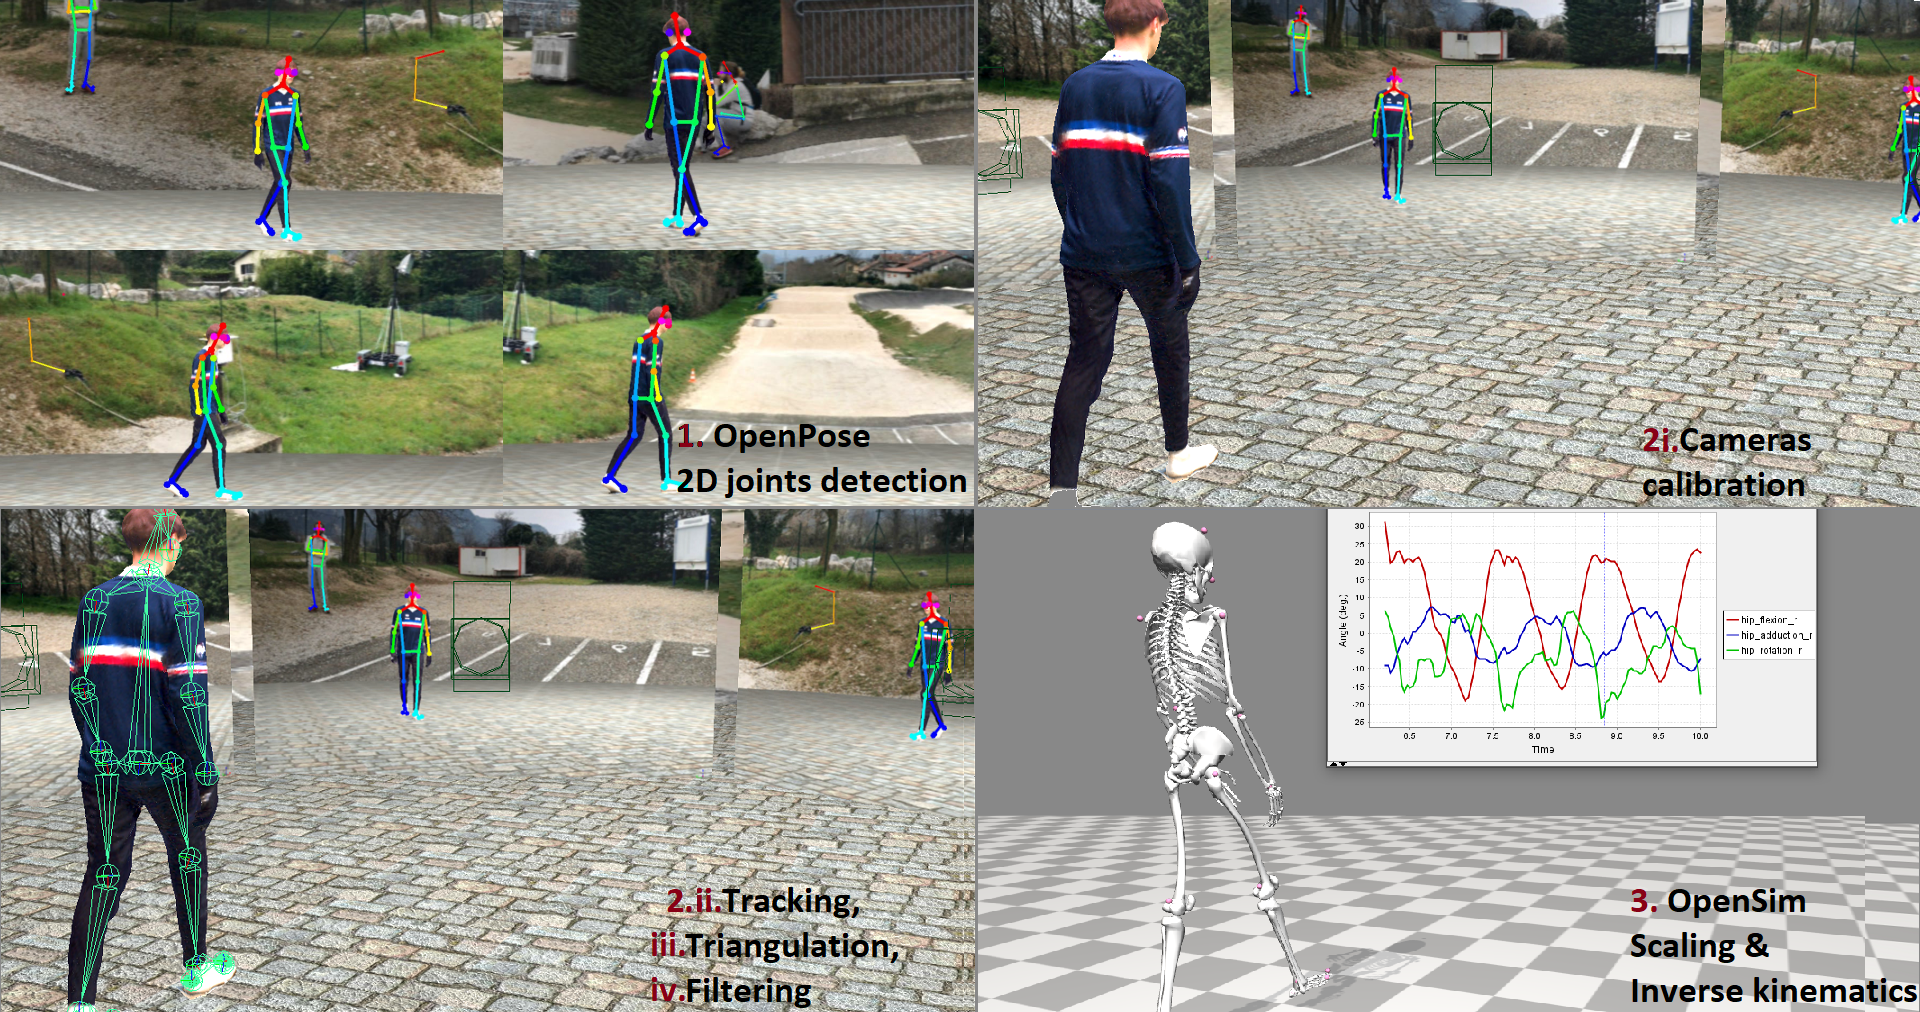
\includegraphics[width=\linewidth]{"../Chap3/Figures/Pipeline.png"}
	\caption{Pose2Sim full pipeline: (1) 2D keypoint detection; (2.1) Camera calibration; \newline(2.1-2.4) Tracking of the person of interest, Triangulating of keypoint coordinates; and Filtering; (3) Constraining the 3D coordinates to an individually scaled, physically consistent OpenSim skeletal model.}
	\label{fig_pipeline}
\end{figure}

\newpage

The repository presents a framework which consists in (Figures~\ref{fig_pipeline}):
\begin{enumerate}[itemsep=0em, topsep=0em, leftmargin=*]
      \item Preliminary 2D joint coordinate detections from multiple videos, e.g. with OpenPose.
      \item Pose2Sim core, including 4 customizable steps:
      \begin{enumerate}[before=\vspace{-0.5\baselineskip}, nosep, label*=\arabic*.]
            \item Camera calibration.
            \item 2D tracking of the person of interest.
            \item 3D keypoint triangulation.
            \item 3D coordinate filtering.
      \end{enumerate}
      \item Scaling a full-body skeleton to each individual subject, and computing inverse kinematics via OpenSim so as to obtain 3D joint angles.
\end{enumerate}

\vskip 1em

Each task is easily customizable, and requires only moderate Python skills. The whole workflow runs from any video cameras, on any computer, equipped with any operating system (although OpenSim has to be compiled from source on Linux.) Pose2Sim has already been used and tested in a number of situations (walking, running, cycling, dancing, balancing, swimming, boxing), and published in peer-reviewed scientific publications assessing the quality of its code \cite{Pagnon2022c}, its robustness (see Chapter 4 on \nameref{ch:4}) \cite{Pagnon2021} and its accuracy (see Chapter 5 on \nameref{ch:5}) \cite{Pagnon2022a}. Its results for inverse kinematics were deemed good when compared to marker-based ones, with errors generally below 4.0° across several activities, on both lower and on upper limbs. The combination of its ease of use, customizable parameters, and high robustness and accuracy makes it promising, especially for "in-the-wild" sports movement analysis.


\section{Installation and demonstration}

\subsection{Installation}

\begin{enumerate}[itemsep=0em, topsep=0em, leftmargin=*]
      \item Install \textbf{OpenPose} (instructions \href{https://github.com/CMU-Perceptual-Computing-Lab/openpose/blob/master/doc/installation/0_index.md}{here}).\newline
      Windows portable demo is enough.
      \item Install \textbf{OpenSim 4.x} from \href{https://simtk.org/frs/index.php?group_id=91}{there}.\newline
      Tested up to v4.4-beta on Windows. Has to be compiled from source on Linux (see \href{https://simtk-confluence.stanford.edu:8443/display/OpenSim/Linux+Support}{there}.
      \item \textit{Optional:} Install \textbf{Anaconda} or \href{https://docs.conda.io/en/latest/miniconda.html}{Miniconda}.\newline
      Open an Anaconda terminal and create a virtual environment by typing:
      \begin{minted}[frame=single, rulecolor=\color{gray!40}, autogobble]{shell-session}
            conda create -n Pose2Sim python=3.8.8
            conda activate Pose2Sim
      \end{minted}
      \item Install \textbf{Pose2Sim}\newline
      If you don't use Anaconda, type \mintinline{shell-session}{python -V} in terminal to make sure python>=3.6 is installed.
      \begin{itemize}
            \item OPTION 1: \textit{Quick install.} Type in terminal:
            \begin{minted}[frame=single, rulecolor=\color{gray!40}, autogobble]{shell-session}
                  pip install pose2sim
            \end{minted}
            \item OPTION 2: \textit{Build from source.} Open a terminal in the directory of your choice and clone the Pose2Sim repository:
            \begin{minted}[frame=single, rulecolor=\color{gray!40}, autogobble]{shell-session}
                  git clone https://gitlab.inria.fr/perfanalytics/pose2sim.git
                  cd pose2sim
                  pip install .
            \end{minted}
      \end{itemize}
\end{enumerate}


\subsection{Demonstration Part-1: Build 3D TRC file on Python}

This demonstration provides an example experiment of a person balancing on a beam, filmed with 4 calibrated cameras processed with OpenPose.

Open a terminal and check package location with  \mintinline{shell-session}{pip show pose2sim | grep Location}. \newline
Copy this path and go to the Demo folder with  \mintinline{shell-session}{cd <path>\pose2sim\Demo`}. \newline
Type \mintinline{shell-session}{python}, and test the following code (Figures~\ref{fig_pose2sim}):
\begin{minted}[frame=single, rulecolor=\color{gray!40}, autogobble]{python}
      from Pose2Sim import Pose2Sim
      Pose2Sim.calibrateCams()
      Pose2Sim.track2D()
      Pose2Sim.triangulate3D()
      Pose2Sim.filter3D()
\end{minted}

You should obtain a plot of all the 3D coordinates trajectories (Figures~\ref{fig_filterplot}). You can check the logs in \mintinline{shell-session}{Demo\Users\logs.txt}. Results are stored as .trc files in the \mintinline{shell-session}{Demo\pose-3d} directory (Figures~\ref{fig_trc}). Note that when the functions are called without any argument, the Config file is searched in the default \mintinline{shell-session}{Users\Config.toml} location. These parameters can be edited by the user.

\begin{figure}[hbtp]
	\centering
	\def\svgwidth{1\columnwidth}
	\fontsize{10pt}{10pt}\selectfont
	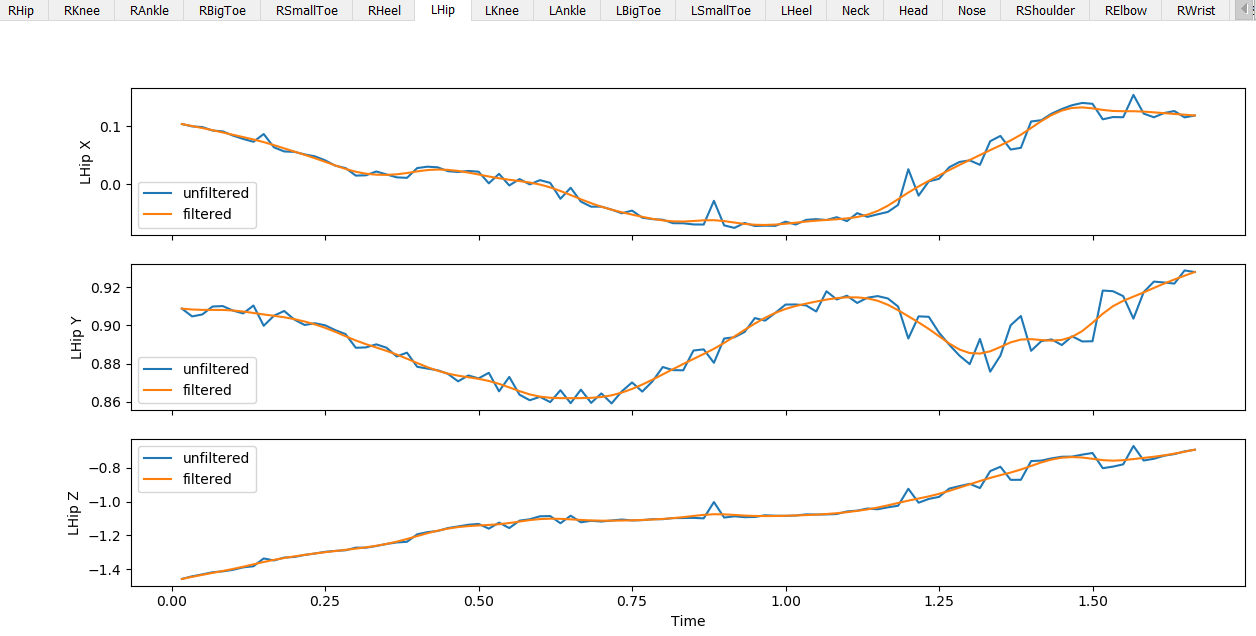
\includegraphics[width=\linewidth]{"../Chap3/Figures/FilterPlot.png"}
	\caption{Filtering results, for each keypoint in a different tab.}
	\label{fig_filterplot}
\end{figure}

\begin{figure}[hbtp]
	\centering
	\def\svgwidth{1\columnwidth}
	\fontsize{10pt}{10pt}\selectfont
	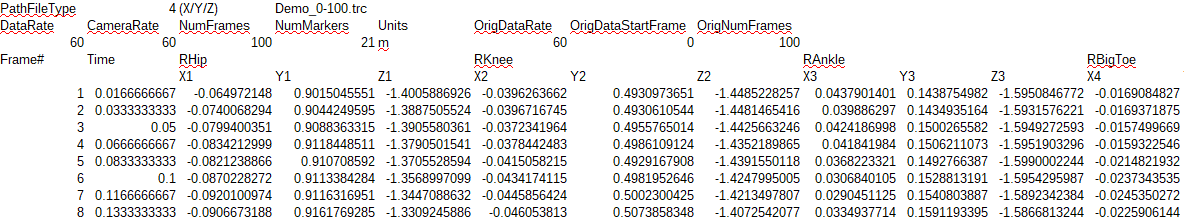
\includegraphics[width=\linewidth]{"../Chap3/Figures/Trc.png"}
	\caption{An example .trc file of triangulated keypoint coordinates, directly usable in OpenSim.}
	\label{fig_trc}
\end{figure}

\begin{figure}[hbtp]
	\centering
	\begin{subfigure}[b]{1\textwidth}
		\centering
		\def\svgwidth{\columnwidth}
		\fontsize{10pt}{10pt}\selectfont
		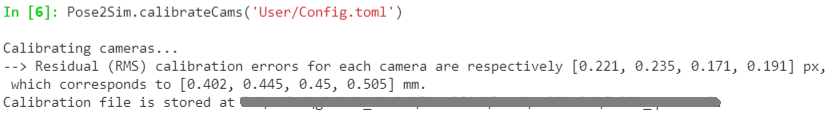
\includegraphics[width=\linewidth]{"../Chap3/Figures/Calib2D.png"}
            \caption{Calibration can either be done from a checkerboard, or by simply converting a Qualisys calibration file. Calibration errors are computed and provided.\newline}
      \end{subfigure}
	\qquad
	\begin{subfigure}[b]{1\textwidth}
		\centering
		\def\svgwidth{\columnwidth}
		\fontsize{10pt}{10pt}\selectfont
		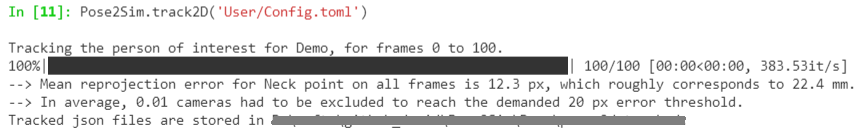
\includegraphics[width=\linewidth]{"../Chap3/Figures/Track2D.png"}
            \caption{If several persons are detected in the scene, a tracking step can be carried out in order to make sure that the right person from each camera will be triangulated.}
      \end{subfigure}
      \begin{subfigure}[b]{1\textwidth}
		\centering
		\def\svgwidth{1\columnwidth}
		\fontsize{10pt}{10pt}\selectfont
		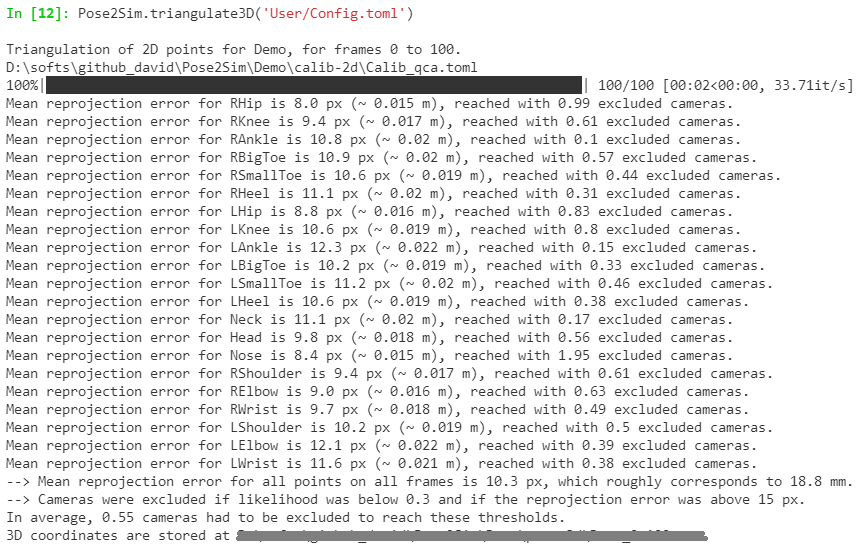
\includegraphics[width=\linewidth]{"../Chap3/Figures/Triangulate3D.png"}
            \caption{The triangulation is weighted by the OpenPose likelihood, and constrained by some thresholds defined in the Config.toml file. If these constraints are not met, e.g., if the reprojection error is too large or if the likelihood of a keypoint is too low, one or several cameras are excluded. The mean reprojection error and the number of cameras that have been excluded to meet the constraints is printed, for each keypoints.}
      \end{subfigure}
      \begin{subfigure}[b]{1\textwidth}
		\centering
		\def\svgwidth{1\columnwidth}
		\fontsize{10pt}{10pt}\selectfont
		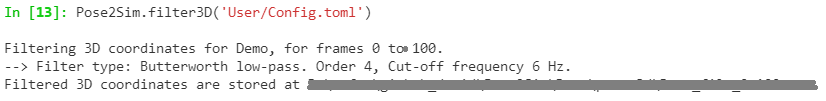
\includegraphics[width=\linewidth]{"../Chap3/Figures/Filter3D.png"}
            \caption{Triangulated data can be filtered, either with a low-pass Butterworth filter or with other types, and parameters can be adjusted.}
      \end{subfigure}
	\caption{First steps of Pose2Sim pipeline in Python. Calibration can either be done from a checkerboard, or by simply converting a Qualisys calibration file. Note that the functions can be used without any arguments if the Config.toml file is left in the default location.}
	\label{fig_pose2sim}
\end{figure}


\FloatBarrier
\subsection{Demonstration Part-2: Obtain 3D joint angles with OpenSim}
In the same vein as we would do with marker-based kinematics, the model first needs to be scaled to each individual, and then inverse kinematics can be performed (Figures~\ref{fig_opensimdemo}).

\textbf{Scaling:}
\begin{enumerate}[itemsep=0em, topsep=0em, leftmargin=*]
      \item Open OpenSim.
      \item Open the provided \mintinline{shell-session}{Model_Pose2Sim_Body25b.osim} model from \mintinline{shell-session}{pose2sim/Demo/opensim}. (File $\mapsto$ Open Model)
      \item Load the provided \mintinline{shell-session}{Scaling_Setup_Pose2Sim_Body25b.xml} scaling file from \mintinline{shell-session}{pose2sim/Demo/opensim}. (Tools $\mapsto$ Scale model $\mapsto$ Load)
      \item Run. You should see your skeletal model take the static pose.
\end{enumerate}

\textbf{Inverse kinematics}
\begin{enumerate}[itemsep=0em, topsep=0em, leftmargin=*]
    \item Load the provided \mintinline{shell-session}{IK_Setup_Pose2Sim_Body25b.xml} scaling file from \mintinline{shell-session}{pose2sim/Demo/opensim}. (Tools $\mapsto$ Inverse kinematics $\mapsto$ Load)
    \item Run. You should see your skeletal model move in the Vizualizer window.
\end{enumerate}

\begin{figure}[hbtp]
	\centering
	\def\svgwidth{1\columnwidth}
	\fontsize{10pt}{10pt}\selectfont
	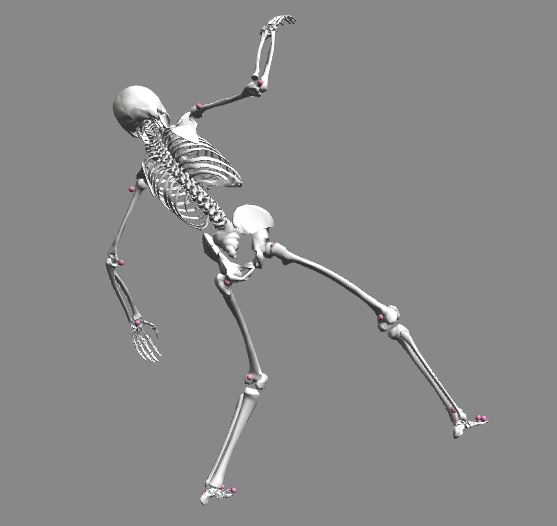
\includegraphics[width=\linewidth]{"../Chap3/Figures/OpenSimDemo.JPG"}
	\caption{At the end of the demonstration, you should have a skeleton balancing on a beam in OpenSim.}
	\label{fig_opensimdemo}
\end{figure}


\section{Method details}

\subsection{Project}
Pose2Sim is meant to be as fully and easily configurable as possible, by editing the \mintinline{shell-session}{User/Config.toml} file. Optional tools are also provided for extending its usage (Figures~\ref{fig_opensimutilities}). First of all, the user can specify the project path and folder names, the video frame rate, and the range of analyzed frames.

\begin{figure}[hbtp]
	\centering
	\def\svgwidth{1\columnwidth}
	\fontsize{10pt}{10pt}\selectfont
	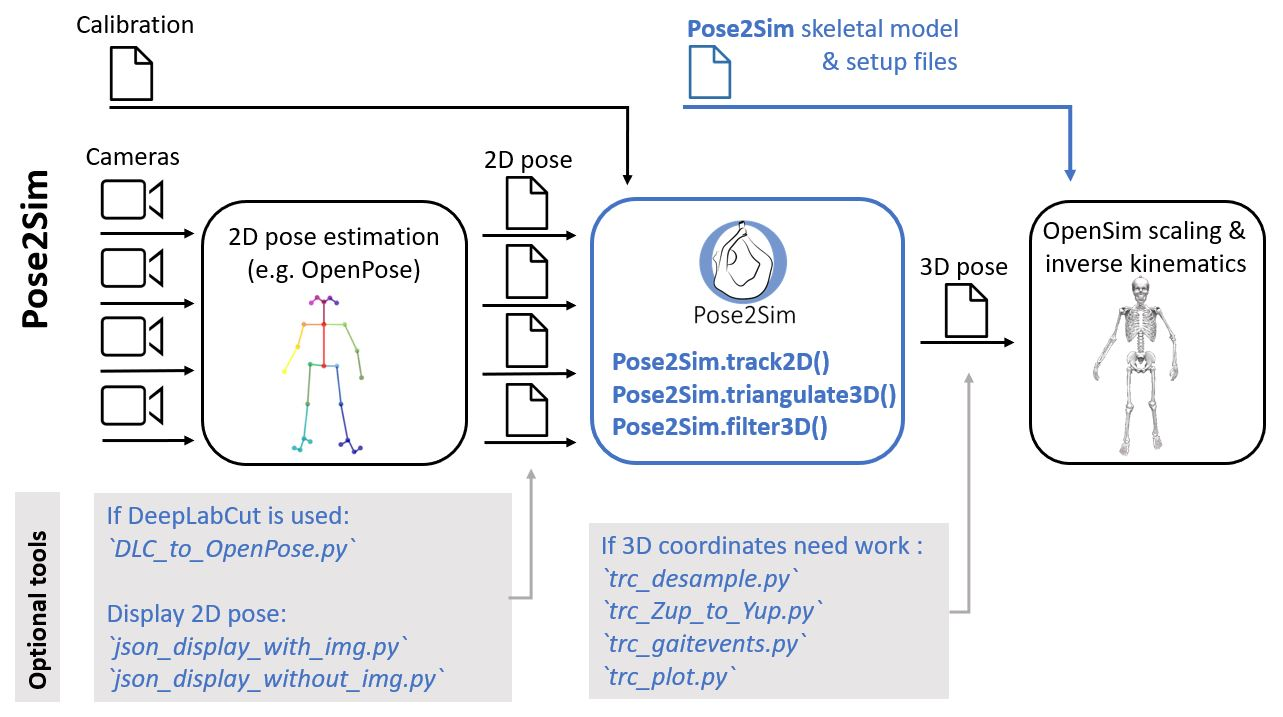
\includegraphics[width=\linewidth]{"../Chap3/Figures/Pose2Sim_utilities.jpg"}
	\caption{The Pose2Sim workflow, along with some optional utilities provided in the package.}
	\label{fig_opensimutilities}
\end{figure}


\subsection{2D keypoint detection}


%The emergence of markerless kinematics opens up new possibilities. Indeed, the interest in deep-learning pose estimation neural networks has been growing fast since 2015 (Zheng et al.,2022), which makes it now possible to collect accurate and reliable kinematic data without the use of physical markers. OpenPose, for example, is a widespread open-source software which provides 2D joint coordinate estimates from videos. 

% need feet: openpose rather than any other potentially faster and more accurate. BlazePose provides feet but single person (and always people in background)


\subsection{Camera calibration}

\subsection{Tracking the person of interest}

\subsection{Triangulating}

% Open source tools for triangulating
% Some tools have been released open source
% Aside from ours (see Chapter 3 on \nameref{ch:3}), a number a tools have been made available for such triangulation: the experimental OpenPose 3D reconstruction module [Hidalgo2021], the FreeMoCap Python and Blender toolbox [Matthis2022], or the pose3d Matlab toolbox [Sheshadri2020]. Yet, when it comes to the biomechanical analysis of human motion, it is often more useful to obtain joint angles than joint center positions in space. Joint angles allow for better comparison among trials and individuals, and they represent the first step for other analyses such as inverse dynamics. EasyMocap ?


\subsection{Filtering and other operations}


\subsection{OpenSim scaling and inverse kinematics}

A full-body OpenSim \cite{Delp2007,Seth2018} skeletal model with OpenPose keypoints is provided, as well as scaling and inverse kinematics setup files.

OpenSim is another widespread open-source software which helps compute 3D joint angles, usually from marker coordinates. It lets scientists define a detailed musculoskeletal model, scale it to individual subjects, and perform inverse kinematics with customizable biomechanical constraints. It provides other features such as net calculation of joint moments or resolution of individual muscle forces, although this is beyond the scope of our contribution.


\section{Limitations and perspectives}
% ajouter video de use on your own data


\section{Helper functions and vizualisation tools}
Maya MoCap
Bath


